\chapter{Experimental Results}\label{ch:expRes}

In the following chapter the different variants of the RLS and the (1+1) EA are now analysed empirically.
Additionally for most lemmas from the previous chapters there are also tests if they actually hold in practice.

\section{Code}
The complete java code used for all empirical studies is available on GitHub:\newline
https://github.com/Err404NameNotFound/PartitionSolvingWithEAs.\newline
\subsection{The Algorithms}
All different variants of the RLS function more or the less the same. They start with an initial random value and then optimise this one value int the loop. The loop can be summarised like this:
\begin{enumerate}
      \item generate a number k of bits to be flipped (algorithm specific)
      \item flip k random bits
      \item evaluate fitness of the mutated individual
      \item replace old value with new value if new value is better
      \item repeat if not optimal
\end{enumerate}
The (1+1) EA variants behave a differently on the first impression as there every bit is flipped independently with probability $c/n$. This can be seen as n independent Bernoulli trials with probability $c/n$. The amount of bits that are flipped is therefore binomial distributed and the algorithm can be implemented exactly as the versions of the RLS. The same hold for the pMut operator which generates a number k with a powerlaw distribution and then flips k bits. This leads to only one implementation of a partition solving algorithm which is not only given the input array of numbers but also a generator for the amount of bits to be flipped in each step. The random values for the amount of bits to be flipped are generated accordingly to this table:

\begin{tabular}{c c}
      Algorithm & Returned value                                                                          \\
      \hline
      RLS       & 1                                                                                       \\
      RLS-N(k)  & $y \in \{1,\dots,k\}$ with probability $\frac{\binom{n}{y}}{\sum_{i=1}^k \binom{n}{i}}$ \\
      RLS-R(k)  & uniform random value $x \in \{1,\dots,k\}$                                              \\
      (1+1) EA  & binomial distributed value from \textasciitilde$B(n,c/n)$                               \\
      pMut      & random value generated from powerlaw distribution with parameter $\beta$                \\
\end{tabular}



\begin{algorithm}[bt]
      \caption{\textsc{GenericPartitionSolver}}\label{alg:genericPartition}

      % Some settings
      \DontPrintSemicolon %dontprintsemicolon
      \SetFuncSty{textsc}

      % The algorithm
      \BlankLine
      choose x uniform from ${\{0,1\}}^n$\;
      \While{$x$ not optimal}
      {
      $x' = x$\;
      $k = \text{kGenerator.generate()}$\;
      flip $k$ uniform random bits of $x'$\;
      {
      \If{$f(x') \le f(x)$}
      {
            $x \leftarrow x'$\;
      }
      }
      }
\end{algorithm}

\section{Do inputs have perfect partitions?}
\subsection{Binomial Inputs}

Lemma~\ref{lemma:BinomialSolvable} is only valid for larger n. In practice the bound is much smaller depending on the expected value of a single value. Another factor deciding how likely an input is to have a perfect partition is if n is even or odd. Here is conducted two experiments. The goal of the first experiment was to determine the influence of the array size to the input having a perfect partition. So for every possible combination of $p \in \{0.1, 0.2, \dots , 0.8, 0.9\}, m \in \{10,100,1000,10^4,10^5\} \text{and} n \in \{2,3,4,\dots,19,20\}$ 1000 randomly generated inputs of size $n$ were generated and tested for a perfect partition. Due to the small values for $n$ it was possible to brute force the results in a short amount of time. The results are visualised in figure~\ref{fig:firstBinPercentage} to figure~\ref{fig:lastBinPercentage}. 
On the x-axis is the size of the input and on the y-axis the percentage of inputs that had a perfect partition. The different graphs in one figure are for the different values of p uses for generating the inputs. The graph for 0.1 resembles the percentage of inputs that had a perfect partition that were generated from the distribution \textasciitilde$B(m,0.1)$ with $m$ being dependent on the figure. For figure~\ref{fig:firstBinPercentage} $m=10$.\newline
It is easy to see that for small inputs sizes it is relevant if n is even or odd as all curves in figure~\ref{fig:lastBinPercentage} oscillate between 0\% and 100\%. Another effect visible is the decreasing percentage with rising p. This may be a direct result of the value chosen for p but can also be an indirect result as the value for p changes the expected value for a constant m. This leads to the second experiment.

\begin{figure}[h]
      \centering
      \begin{minipage}[b]{0.45\textwidth}
            \caption{Percentage of Binomial inputs with perfect partitions for m = 10}
            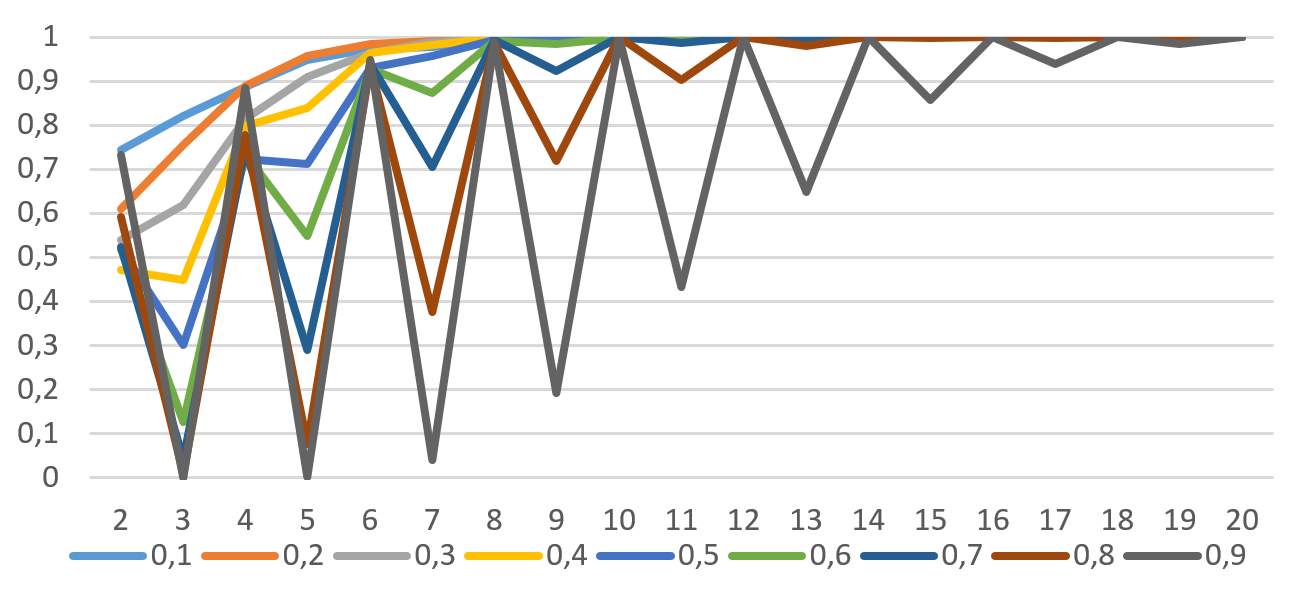
\includegraphics[width=\textwidth]{figures/images/solvabilityOfInputs/binomial_Input_Solvable_m10.png}\label{fig:firstBinPercentage}
      \end{minipage}
      \hspace{0.75cm}
      \begin{minipage}[b]{0.45\textwidth}
            \caption{Percentage of Binomial inputs with perfect partitions for m = 100}
            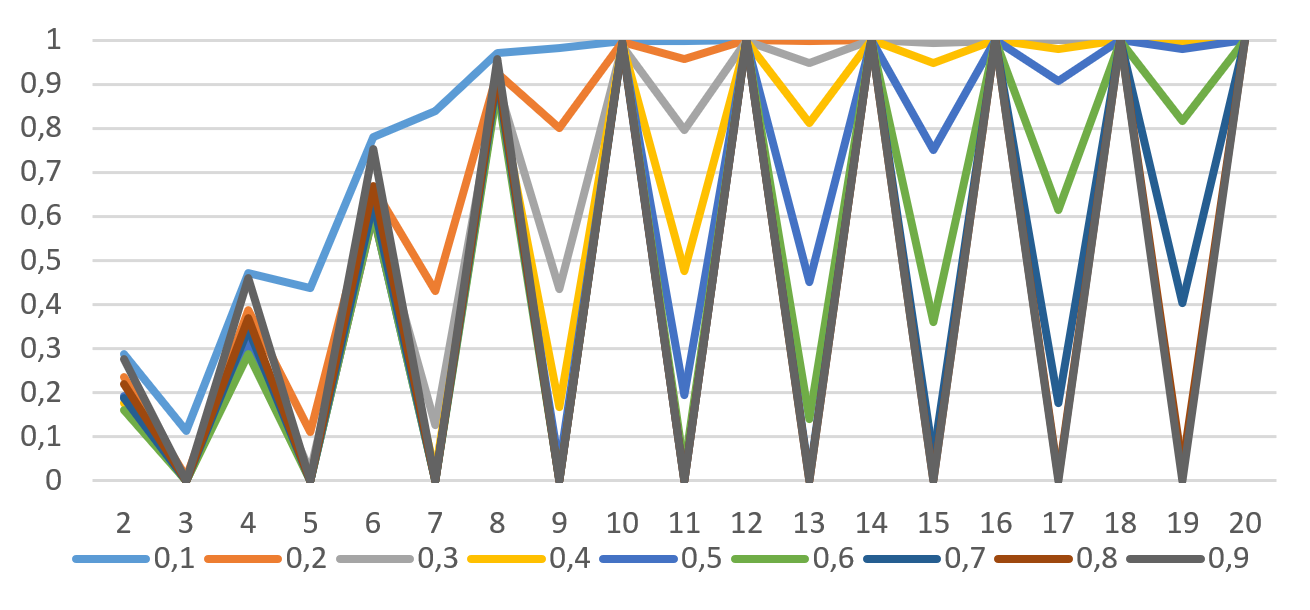
\includegraphics[width=\textwidth]{figures/images/solvabilityOfInputs/binomial_Input_Solvable_m100.png}
      \end{minipage}
\end{figure}

\begin{figure}[h]
      \centering
      \begin{minipage}[b]{0.45\textwidth}
            \caption{Percentage of Binomial inputs with perfect partitions for m = 1000}
            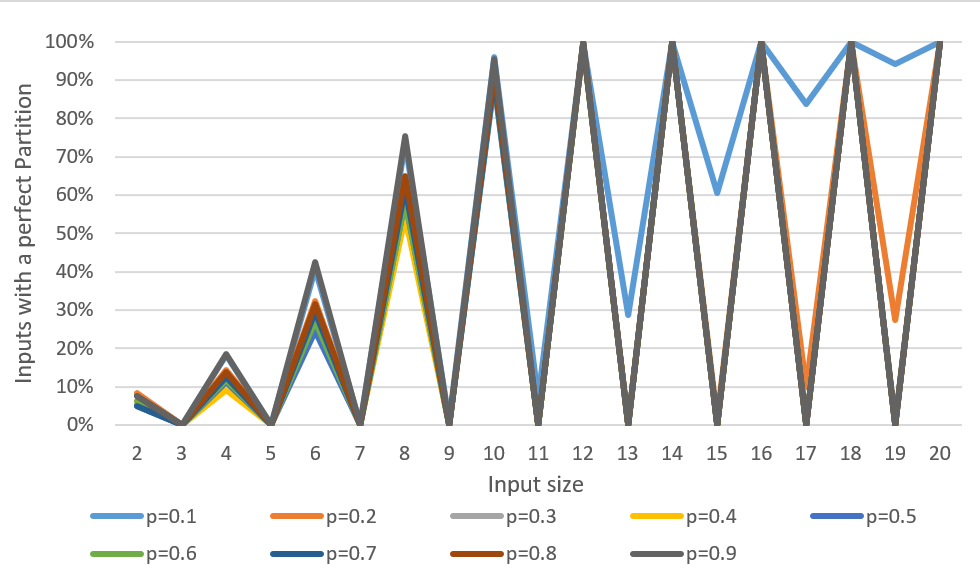
\includegraphics[width=\textwidth]{figures/images/solvabilityOfInputs/binomial_Input_Solvable_m1000.png}
      \end{minipage}
      \hspace{0.75cm}
      \begin{minipage}[b]{0.45\textwidth}
            \caption{Percentage of Binomial inputs with perfect partitions for m = 10000}
            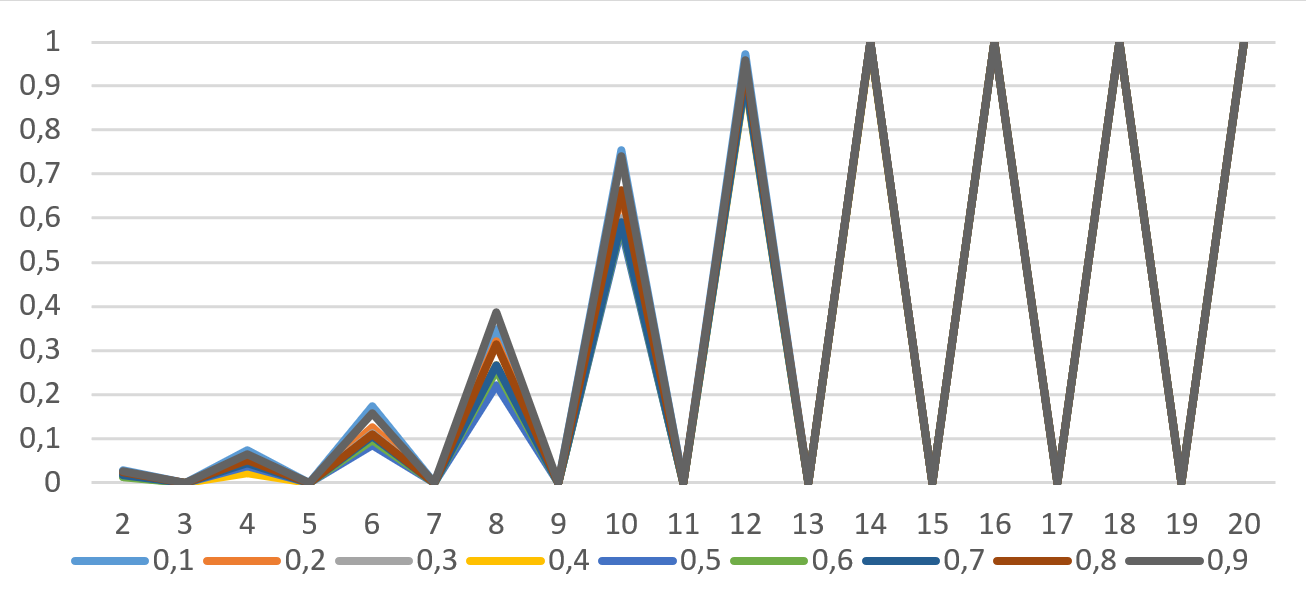
\includegraphics[width=\textwidth]{figures/images/solvabilityOfInputs/binomial_Input_Solvable_m10000.png}
      \end{minipage}
\end{figure}

\begin{figure}[h]
      \caption{Percentage of Binomial inputs with perfect partitions for m = 100000}
      \centering
      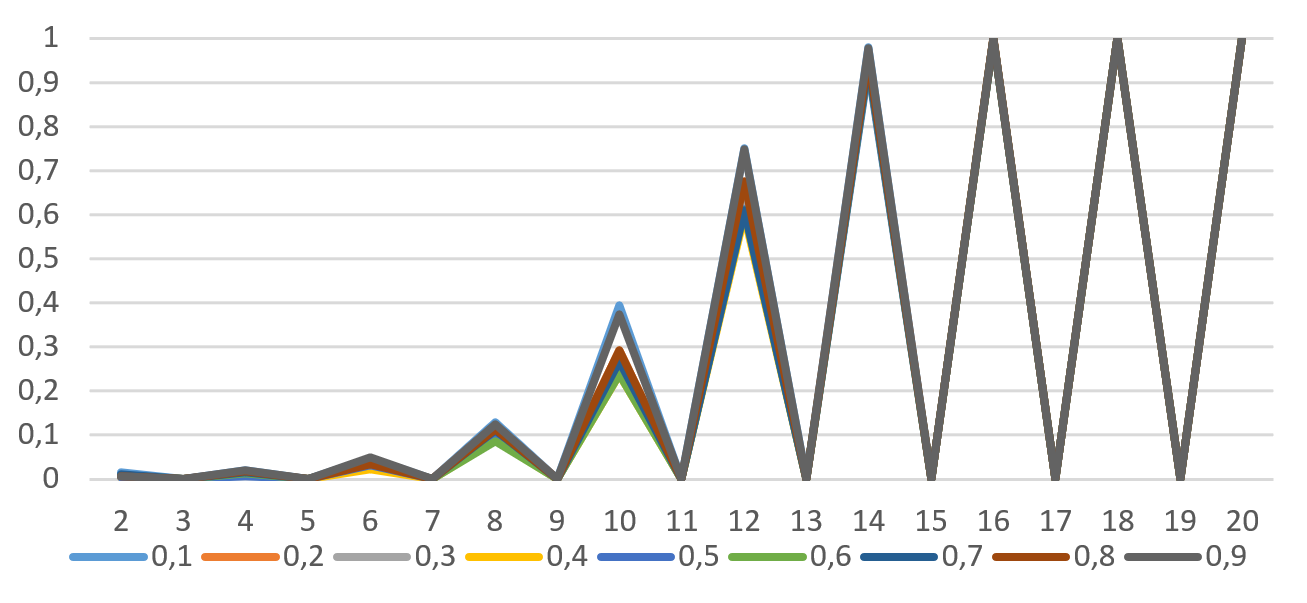
\includegraphics[width=0.45\textwidth]{figures/images/solvabilityOfInputs/binomial_Input_Solvable_m100000.png}\label{fig:lastBinPercentage}
\end{figure}


In the second experiment the inputs were generated a bit differently. Here the goal was to keep the expected value fixed for any combination of $p$ and $n$ and set the value of $m$ to $e/p$ for all $e \in \{10, 20, 30, 40, 50, 100, 200, 500, 1000, 2000, 5000, 10000, 50000\}$. With this setup the influence of the expected value is almost isolated from the other parameters. The probability is still linked $p$ as p also influences the variance $mp(1-p)$. By looking at figure~\ref{fig:firstBinPercentage2} to figure~\ref{fig:lastBinPercentage2} it seems as if the value of $p$ has a much smaller influence than the expected value.

\begin{figure}[h]
      \centering
      \begin{minipage}[b]{0.45\textwidth}
            \caption{Percentage of Binomial inputs with perfect partitions for p = 0.1}
            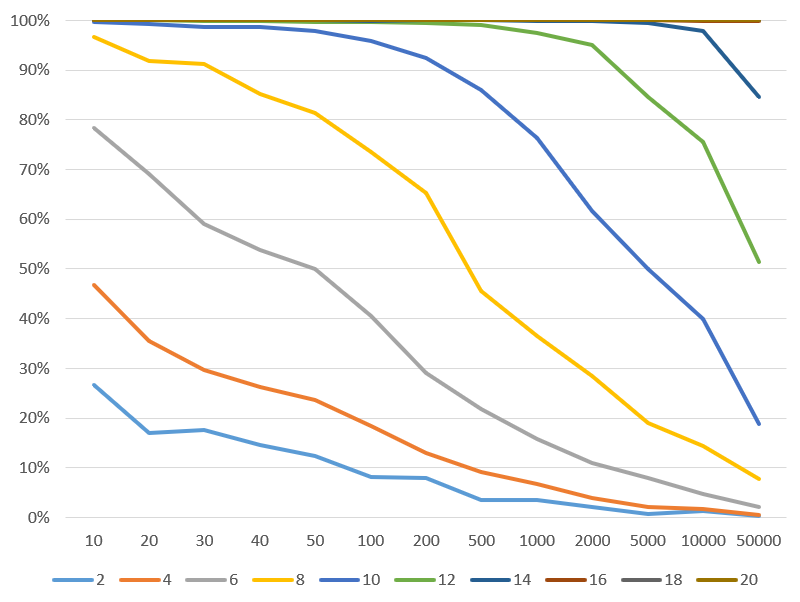
\includegraphics[width=\textwidth]{figures/images/solvabilityOfInputs/solvability0_1.png}\label{fig:firstBinPercentage2}
      \end{minipage}
      \hspace{0.75cm}
      \begin{minipage}[b]{0.45\textwidth}
            \caption{Percentage of Binomial inputs with perfect partitions for p = 0.2}
            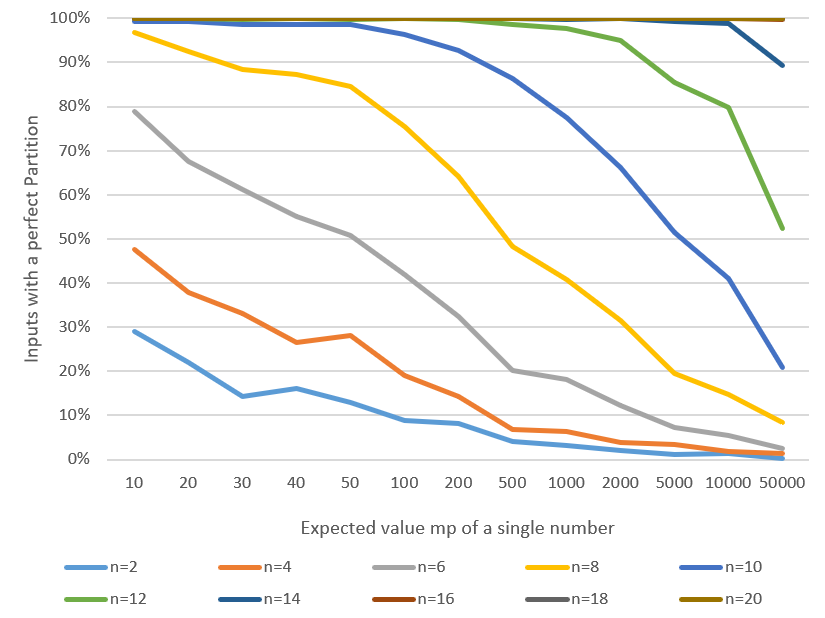
\includegraphics[width=\textwidth]{figures/images/solvabilityOfInputs/solvability0_2.png}
      \end{minipage}
\end{figure}


\begin{figure}[h]
      \centering
      \begin{minipage}[b]{0.45\textwidth}
            \caption{Percentage of Binomial inputs with perfect partitions for p = 0.3}
            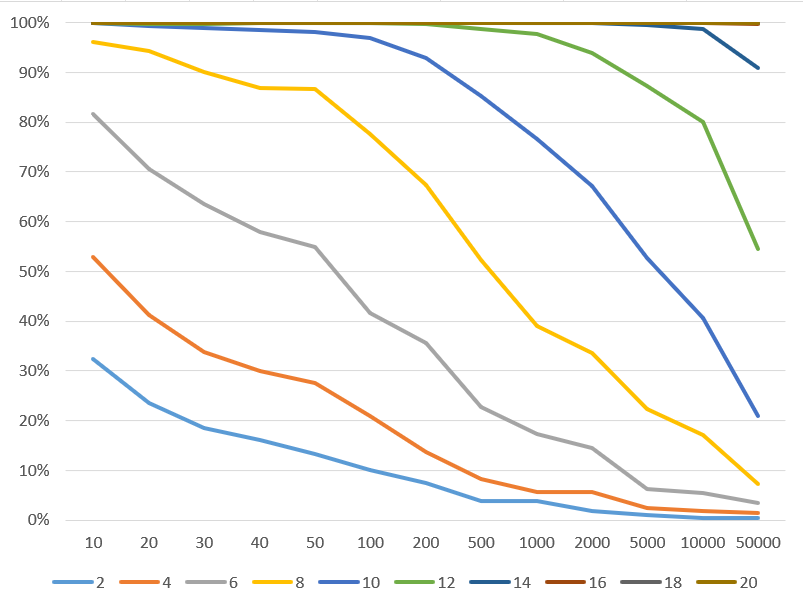
\includegraphics[width=\textwidth]{figures/images/solvabilityOfInputs/solvability0_3.png}
      \end{minipage}
      \hspace{0.75cm}
      \begin{minipage}[b]{0.45\textwidth}
            \caption{Percentage of Binomial inputs with perfect partitions for p = 0.4}
            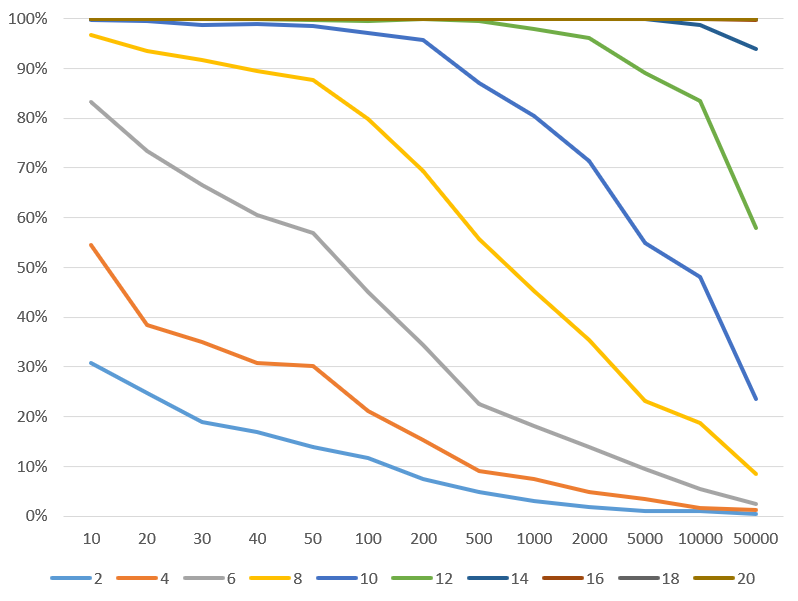
\includegraphics[width=\textwidth]{figures/images/solvabilityOfInputs/solvability0_4.png}
      \end{minipage}
\end{figure}


\begin{figure}[h]
      \centering
      \begin{minipage}[b]{0.45\textwidth}
            \caption{Percentage of Binomial inputs with perfect partitions for p = 0.5}
            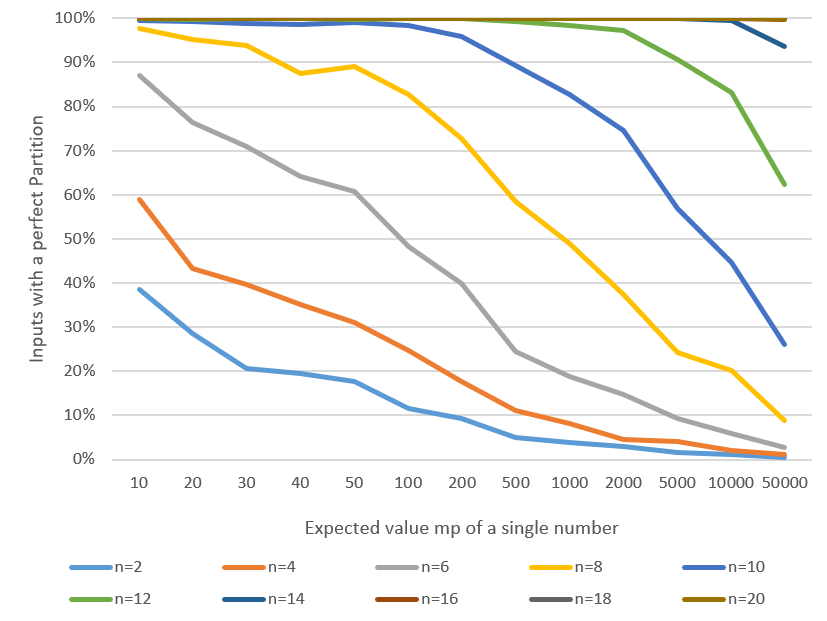
\includegraphics[width=\textwidth]{figures/images/solvabilityOfInputs/solvability0_5.png}
      \end{minipage}
      \hspace{0.75cm}
      \begin{minipage}[b]{0.45\textwidth}
            \caption{Percentage of Binomial inputs with perfect partitions for p = 0.9}
            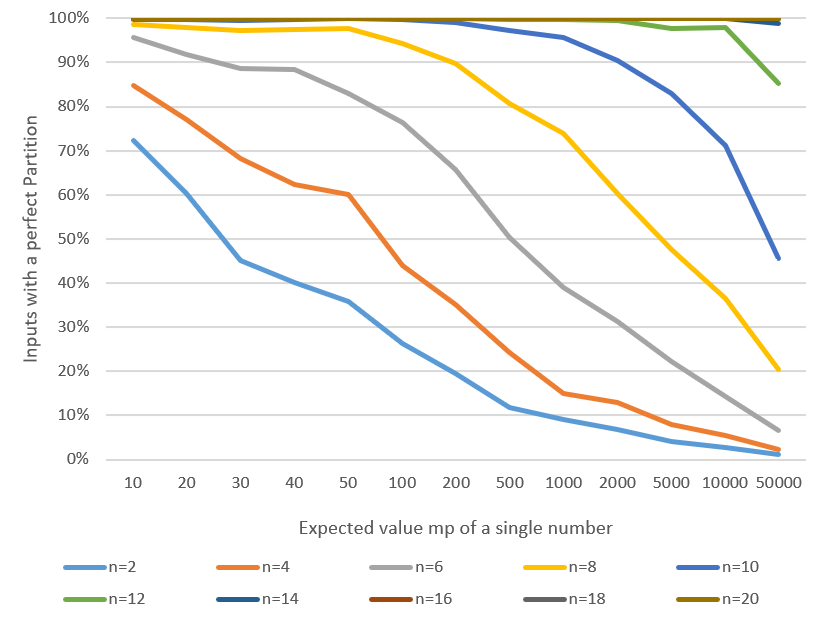
\includegraphics[width=\textwidth]{figures/images/solvabilityOfInputs/solvability0_9.png}\label{fig:lastBinPercentage2}
      \end{minipage}
\end{figure}

\section{Binomial distributed inputs}
\subsection{RLS Comparison}
\subsection{(1+1) EA Comparison}
\subsection{pmut Comparison}
\subsection{Comparison of the best variants}

\section{Uniform distributed inputs}
\subsection{RLS Comparison}
\subsection{(1+1) EA Comparison}
\subsection{pmut Comparison}
\subsection{Comparison of the best variants}

\section{Exponential distributed inputs}
\subsection{RLS Comparison}
\subsection{(1+1) EA Comparison}
\subsection{pmut Comparison}
\subsection{Comparison of the best variants}

\section{OneMax Equivalent for PARTITION}
This kind of input is more or less equivalent to the OneMax problem. All values except the last are either 1 or uniform
random in any intervall. The last value is the sum of all other values. The optimal solution is therefore the 000...01 or
the 111...01 string. So the best solution is almost identical to OneMax. In the previous chapter the O(nlogn) bound was
proven for the (1+1) EA and the RLS. This seems to hold in practice:
TODO: insert Graph showing RLS and (1+1) EA need time O(nlogn)

For OneMax the mutation rate of 1/n is proven to be optimal for the (1+1) EA (TODO insert cite). This seems to be also
true for the equivalent for PARTITION. For Both the (1+1) EA and both new Variants of the RLS
\subsection{RLS Comparison}
The
\subsection{(1+1) EA Comparison}
\subsection{pmut Comparison}
\subsection{Comparison of the best variants}

\section{Carsten Witts worst case input}
\subsection{RLS Comparison}
\subsection{(1+1) EA Comparison}
\subsection{pmut Comparison}
\subsection{Comparison of the best variants}

\section{PowerLawDistributed}
\subsection{RLS Comparison}
\subsection{(1+1) EA Comparison}
\subsection{pmut Comparison}
\subsection{Comparison of the best variants}

\section{Multiple distributions overlapped}
\subsection{RLS Comparison}
\subsection{(1+1) EA Comparison}
\subsection{pmut Comparison}
\subsection{Comparison of the best variants}

\section{Multiple distributions mixed}
\subsection{RLS Comparison}
\subsection{(1+1) EA Comparison}
\subsection{pmut Comparison}
\subsection{Comparison of the best variants}

\section{Multiple distributions mixed \& overlapped}
\subsection{RLS Comparison}
\subsection{(1+1) EA Comparison}
\subsection{pmut Comparison}
\subsection{Comparison of the best variants}